%%==================================================================%%
%% Author : Tejedo Gonz�lez, Daniel                                 %%
%%          S�nchez Barreiro, Pablo                                 %%
%% Version: 1.0, 18/11/2012                                         %%                   %%                                                                  %%
%% Memoria del Proyecto Fin de Carrera                              %%
%% Antecedentes, archivo ra�z                                       %%
%%==================================================================%%

\chapterheader{Antecedentes}{Antecedentes}
\label{chap:background}

Este cap�tulo trata de describir a grandes rasgos las t�cnicas, tecnolog�as y herramientas utilizadas para la creaci�n de nuestro entorno de especificaci�n y validaci�n de restricciones. El cap�tulo comienza describiendo m�s en detalle lo que es la Ingenier�a de Lenguajes Dirigida Por Modelos, para a continuaci�n presentar las dos principales herramientas de modelaci�n que han sido utilizadas: Ecore y EMFText. M�s adelante se hablar� tambi�n en detalle de los �rboles de caracter�sticas, y por �ltimo se describir� brevemente el entorno de desarrollos de plugins de Eclipse que se utiliz� para implementar diversas funciones de nuestro editor.

\chaptertoc

\section{Ingenier�a de Lenguajes Dirigida por Modelos}
\label{sec:back:ildm}
%%==================================================================%%
%% Author : Tejedo Gonz�lez, Daniel                                 %%
%%          S�nchez Barreiro, Pablo                                 %%
%% Version: 1.0, 18/11/2012                                         %%                   %%                                                                  %%
%% Memoria del Proyecto Fin de Carrera                              %%
%% Antecedentes, Ingenier�a de lenguajes dirigidos por modelos                            %%
%%==================================================================%%

La Ingenier�a de Lenguajes Dirigida por Modelos no es m�s que un caso concreto de la m�s gen�rica Ingenier�a Dirigida por Modelos (o Model-Driven Architecture o MDA) aplicado desde el punto de vista de la Teor�a de Lenguajes Formales, con lo cual es conveniente explicar en qu� consiste MDA y comentar los a�adidos que introduce el enfoque gram�tico.

La Inginier�a Dirigida por Modelos intenta definir la funcionalidad de el sistema que pretendemos crear a trav�s de la creaci�n de uno o varios metamodelos que representen todas las caracter�sticas de nuestro sistema y todas las operaciones que puede llevar a cabo. El principal objetivo de la Ingenier�a Dirigida por Modelos es elevar el nivel de abstracci�n a�n m�s, situ�ndolo por encima del l�mite establecido por los Lenguajes de Alto Nivel. 

El nivel de abstracci�n y complejidad de nuestros metamodelos variar� dependiendo de la cantidad de ellos que incorporemos al sistema. De este modo, un metamodelo que represente todo el sistema directamente ser� m�s dif�cil de entender a primera vista que varios metamodelos que implementen cada uno un tipo de operaci�n o funcionalidad del sistema.

La transformaci�n de esos modelos a c�digo permite la automatizaci�n de tareas que pueden resultar triviales y/o repetitivas al programador, en las cuales de otro modo se invierte mucho tiempo de programaci�n y de detecci�n y depuraci�n de errores. 

Una vez que tengamos los metamodelos necesarios para definir el comportamiento de nuestro sistema, podremos instanciarlos para crear modelos que representen sistemas concretos. Una instancia de un metamodelo es un modelo que cumple todos los requisitos marcados por su metamodelo, y que da valor a los par�metros del mismo (por ejemplo a sus atributos).

La figura \ref{fig1} es un ejemplo de un metamodelo sencillo que represente un constructor de grafos unidireccionales con pesos. O dicho de otro modo, representa la sintaxis abstracta de nuestro sistema. Se denomina modelo de sintaxis abstracta a cualquier metamodelo que represente los conceptos y el comportamiento del sistema, y cuyas instancias representen elementos reconocibles dentro de ese sistema.

\begin{figure}[t]
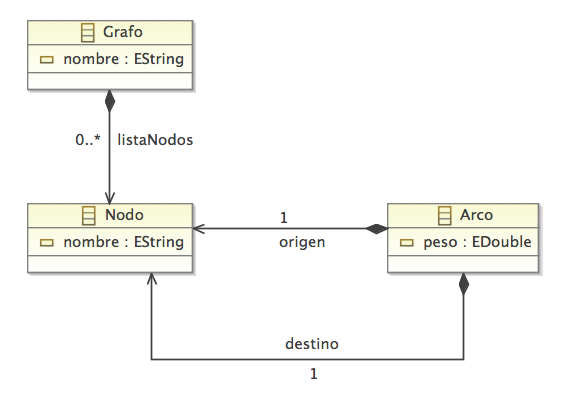
\includegraphics[scale=0.5]{background/abstracta.jpg}
\caption{Metamodelo (sintaxis abstracta) de un creador de grafos}
\label{fig1}
\end{figure}

En el ejemplo presentado, el metamodelo presenta la sintaxis abstracta de nuestro sisstema porque cualquier instanciaci�n v�lida del mismo constituye un grafo completo. Dentro del contexto particular de la Ingenier�a de Lenguajes Dirigida por Modelos, la sintaxis abstracta representa cualquier conjunto de l�neas de c�digo v�lidas que pueden construirse a partir de ella, y posteriormente ser ejecutadas.

Explicando el metamodelo de nuestro ejemplo un poco m�s en detalle, podemos decir que la clase Grafo representa el conjunto final de un grafo construido, y puede tener varios Nodos. Esos nodos, a su vez, pueden estar conectados por Arcos. Cada arco tiene un origen, un destino y un peso. Cualquier instanciaci�n de este metamodelo representa un grafo completo.

La figura \ref{fig2} muestra un ejemplo de instanciaci�n del metamodelo anterior. Esta instancia representa un grafo sencillo que muestra las distancias entre algunas ciudades. O dicho de otro modo, es una de las m�ltiples sintaxis concretas que podemos construir a partir de nuestra sintaxis abstracta. 

\begin{figure}[t]
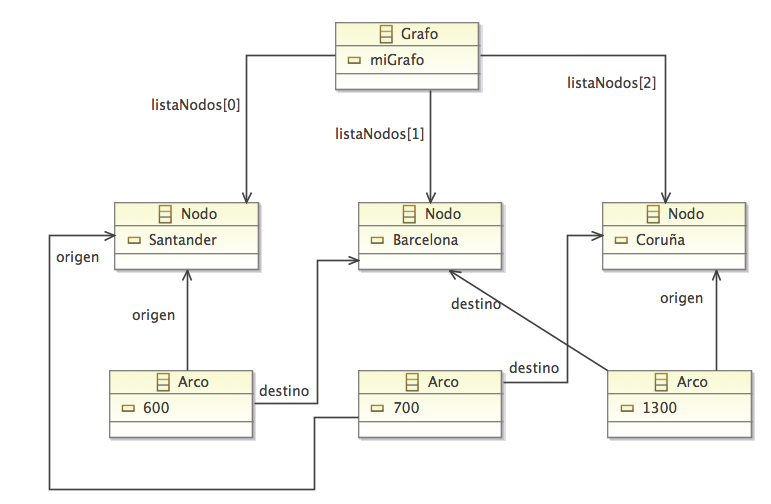
\includegraphics[scale=0.5]{background/concreta.jpg}
\caption{Instancia del metamodelo (sintaxis concreta) que representa un grafo espec�fico}
\label{fig2}
\end{figure}

Dentro del marco de la Ingenier�a de Lenguajes Dirigida por Modelos, una sintaxis concreta es cualquier conjunto de expresiones v�lidas que hayan sido generadas con nuestra sintaxis abstracta. Pero no s�lo eso, el hecho de que estemos trabajando con lenguajes conlleva irrevocablemente el tener que desarrollar una gram�tica de producciones para poder construir nuestras l�neas de c�digo en el orden apropiado y con los s�mbolos apropiados. Eso s�, la gram�tica ser� m�s sencilla y comprensible que la que habr�a que construir de no estar usando este tipo de metodolog�a. Esta tarea tambi�n queda englobada en la sintaxis concreta. De este modo, la sintaxis concreta se suele clasificar en sintaxis concreta visual (el modelo, expresado mediante l�neas de c�digo en el caso de lenguajes, o un grafo pintado en el caso del ejemplo mostrado) y sintaxis concreta textual (la gram�tica del lenguaje).

La figura \ref{fig3} muestra una sintaxis concreta visual del grafo de la figura \ref{fig2}.

\begin{figure}[t]
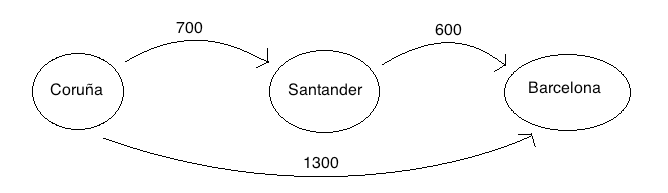
\includegraphics[scale=0.5]{background/grafo.jpg}
\caption{Sintaxis visual del grafo de la figura \ref{fig2}}
\label{fig3}
\end{figure}

Una vez que hemos completado estos pasos, s�lamente queda dotar al sistema de una sem�ntica, es decir, de un comportamiento en ejecuci�n. En el ejemplo de nuestro generador de grafos podr�amos crear una sem�ntica para calcular distancias m�nimas entre caminos. En el caso concreto de la Ingenier�a de Lenguajes Dirigida por Modelos esta sem�ntica representa el comportamiento de las l�neas de c�digo cuando son ejecutadas. Por poner un ejemplo sencillo, es la encargada de que la instrucci�n "4 < 5" compruebe si efectivamente el 4 es menor que el 5.

Una vez se han explicado las bases de la Ingenier�a de Lenguajes Dirigida por Modelos vamos a proceder a mostrar y explicar muy brevemente el metamodelo usado para generar las estructuras v�lidas de c�digo para el lenguaje de especificaci�n y validaci�n de restricciones que hemos creado en este PFC. Ese metamodelo corresponde a la figura \ref{fig4}

\begin{figure}[t]
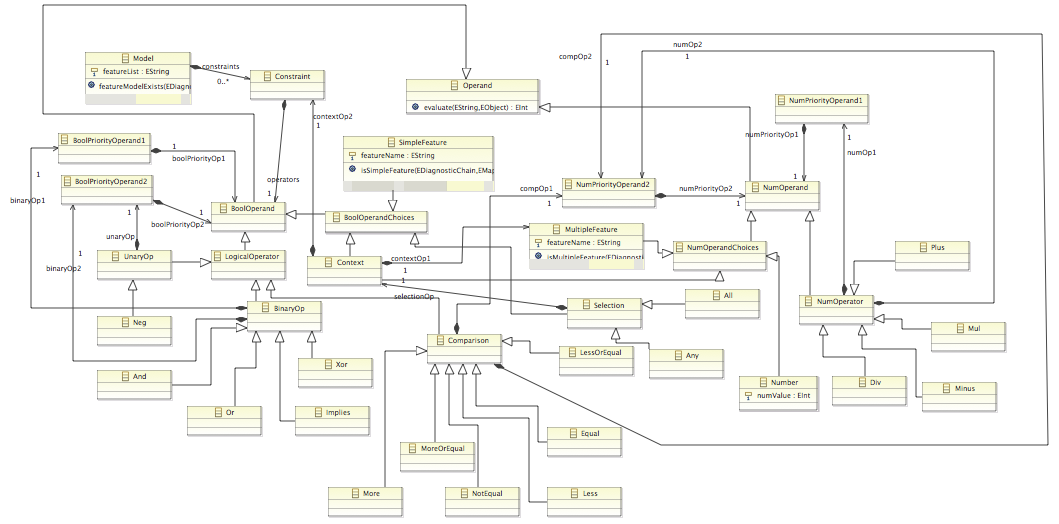
\includegraphics[scale=0.4]{background/metamodelo.jpg}
\caption{Metamodelo utilizado para la creaci�n de nuestro lenguaje de especificaci�n y validaci�n de restricciones}
\label{fig4}
\end{figure}

La clase que engloba todo el conjunto resultante es Model. Un modelo puede tener varias restricciones, y estas a su vez pueden tener varias operaciones booleanas (ya que una restricci�n siempre tiene que evaluarse a true o false). Esas operaciones booleanas se dividen en varios tipos: unarias (negaci�n) , binarias (and, or, etc.), de comparaci�n ( mayor que, menor que, etc.). o de selecci�n (all, any)  Los operandos pueden ser otras operaciones o caracter�sticas (en ingl�s Features). M�s adelante se explicar� en detalle la sintaxis del lenguaje creado.









 

\section{EMF, Ecore y EMF Validation Framework}
\label{sec:back:ecore}
%%==================================================================%%
%% Author : Tejedo Gonz�lez, Daniel                                 %%
%%          S�nchez Barreiro, Pablo                                 %%
%% Version: 1.0, 18/11/2012                                         %%                  
%%                                                                  %%
%% Memoria del Proyecto Fin de Carrera                              %%
%% Antecedentes, ecore                                              %%
%%==================================================================%%

EMF \emph{Eclipse Modeling Framework}~\cite{} es un \emph{plug-in} para Eclipse~\cite{} que permite elaborar metamodelos. Pera ello proporciona un lenguaje de metamodelo denominado Ecore, el cual se ha convertido en el est�ndar de factor para la realizaci�n de metamodelos. Utilizando Ecore se pueden crear metamodelos de forma gr�fica usando una notaci�n muy similar a la los diagramas de clases de UML. La Figura~\ref{fig:sle:metamodeloGrafo} muestra un sencillo ejemplo de metamodelo en Ecore (ver Secci�n~\ref{sec:intr:sle} para m�s detalles). EMF tambi�n incorpora una herramienta para la validaci�n reglas adicionales que no puedan ser especificadas a nivel de del metamodelo. 
 
EMF permite que, a partir de un metamodelo especificado en Ecore, podamos, utilizando diversos generadores de c�digo, crear autom�ticamente un conjunto de clases que nos permiten manipular dichos modelos a nivel de c�digo. Dichas clases se pueden adem�s distribuir como \emph{plug-in} para el entorno Eclipse.

Adem�s, al haberse convertido en est�ndar \emph{de facto} para el desarrollo de metamodelos, Ecore es compatible con multitud de herramientas para Ingenier�a de Lenguajes Dirigida por Modelos, como EMFText, la cual se describe en la siguiente secci�n, o diversos generadores de c�digo o herramientas de transformaci�n de modelos. 



\section{EMFText}
\label{sec:back:emftext}
%%==================================================================%%
%% Author : Tejedo Gonz�lez, Daniel                                 %%
%%          S�nchez Barreiro, Pablo                                 %%
%% Version: 1.0, 18/11/2012                                         %%                   %%                                                                  %%
%% Memoria del Proyecto Fin de Carrera                              %%
%% Antecedentes, emftext                                      %%
%%==================================================================%%


EMFText es una herramienta espec�ficamente dise�ada para dise�ar las gram�ticas de los lenguajes que hayan sido dise�ados previamente con un metamodelo de Ecore. Est� especializado para la creaci�n de Lenguajes Espec�ficos de Dominio, aunque tambi�n se pueden crear lenguajes de prop�sito general. 

Pero, como en casi todos los casos de este tipo de herramientas, su mayor virtud es la enorme cantidad de c�digo autogenerado que produce, y que elimina al programador de tareas tediosas que adem�s en muchos casos podr�an resultar complicadas. Todo el c�digo generado es completamente independiente de EMFText, es decir, podr� ser ejecutado en plataformas que no tengan la herramienta instalada. 

Todo el c�digo generado por EMFText est� dise�ado de tal modo que sea f�cil de modificar en caso de que queramos poner en pr�ctica algunas funcionalidades poco habituales. Se facilita mucho la labor a la hora de modificar estructuras como el postprocesador de nuestra gram�tica. Todas las gram�ticas construidas tendr�n que ser LL por defecto, a no ser que queramos modificar los parsers generados, posibilidad tambi�n disponible. 

Otro tipo de funcionalidades implementadas, quiz�s no tan importantes pero tambi�n de gran utilidad, son el coloreado de c�digo (por defecto o personalizable), funci�n de completar c�digo, generaci�n del �rbol parseado en el la vista de eclipse Outline o generaci�n de c�digo para crear un depurador para nuestro lenguaje.

\begin{figure}[t]
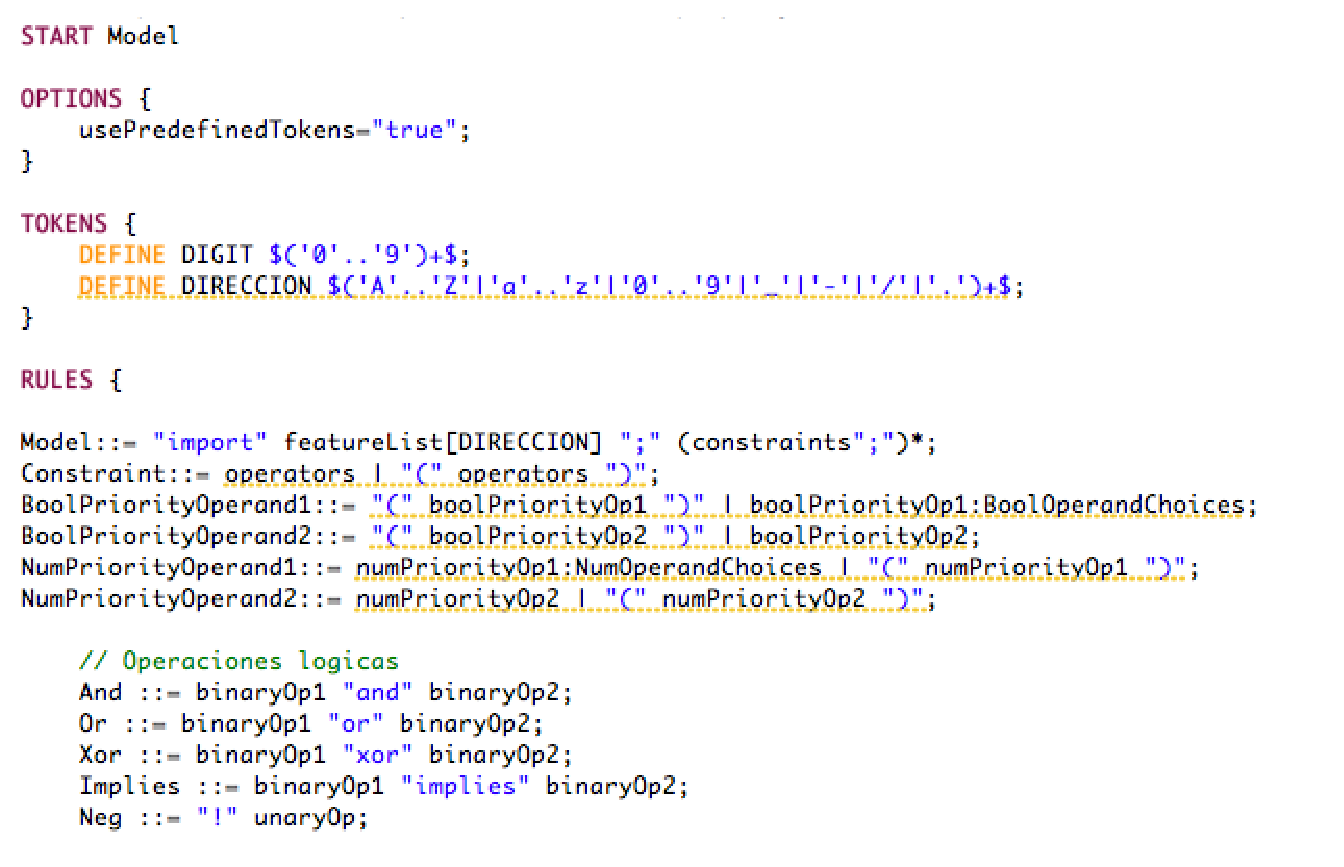
\includegraphics[scale=0.5]{background/gramatica.eps}
\caption{Trozo de la gram�tica de nuestro editor de especificaci�n y validaci�n de restricciones}
\label{fig5}
\end{figure}


EMFText permite la definici�n de gram�ticas utilizando un lenguaje est�ndar para la definici�n de expresiones regulares, adem�s de incorporar algunas particularidades propias que facilitan ciertas tareas. En la figura \ref{fig5} se muestra una peque�a captura que contiene una porci�n de la gram�tica construida para nuestro editor de especificaci�n y validaci�n de restricciones. 

\section{�rboles de caracter�sticas}
\label{sec:back:fmodels}
%%==================================================================%%
%% Author : Tejedo Gonz�lez, Daniel                                 %%
%%          S�nchez Barreiro, Pablo                                 %%
%% Version: 1.0, 18/11/2012                                         %%                   
%% Version: 2.0, 05/02/2013                                         %%                   
%%                                                                  %%
%% Memoria del Proyecto Fin de Carrera                              %%
%% Antecedentes, �rboles de caracter�sticas                         %%
%%==================================================================%%

Como se ha comentado en la secci�n anterior, una de las tareas clave para el �xito de una l�nea de productos software consiste en analizar la variabilidad existente en la familia de productos software que dicha l�nea de productos software pretende cubrir. Aqu� es donde entran en juego los \emph{�rboles de caracter�sticas}~\cite{kang:1990, czarnecky:2005, danilo:2003}. Una \emph{caracter�stica} se define como ``\emph{un incremento en la funcionalidad del producto}'', o m�s formalmente, ``\emph{una caracter�stica es una propiedad de un sistema que es relevante a algunos \emph{stakeholders} y que es utilizada para capturar propiedades comunes o diferenciar entre sistemas de una misma familia}''~\cite{eisenecker:2000}. De este modo un producto queda representado por las caracter�sticas que posee.

Para poder capturar las divergencias y aspectos comunes entre los distintos productos de una misma familia, los �rboles de caracter�sticas organizan de forma jer�rquica el conjunto de caracter�sticas que posee una familia de productos. Cada caracter�stica se representa como un nodo en el �rbol de caracter�sticas. La ra�z de dicho �rbol es siempre el sistema o producto software cuya variabilidad estamos analizando. Cada caracter�stica se puede descomponer en varias subcaracter�sticas, siendo est�s �ltimas nodos \emph{hijos} de la primera caracter�stica, que actuar�a como \emph{padre}. Dependiendo de si dichas subcaracter�sticas son obligatorias, alternativas u opcionales, existen diversos tipos de relaciones padre-hijo. 

%%=========================================================================================%%
%% NOTA(Pablo): Para esta figura, hazte un modelo para la Smart Home sin habitaciones ni   %%
%%              plantas. Lo puedes encontrar en un art�culo que te mando luego             %% %%=========================================================================================%%
\begin{figure}[!tb]
    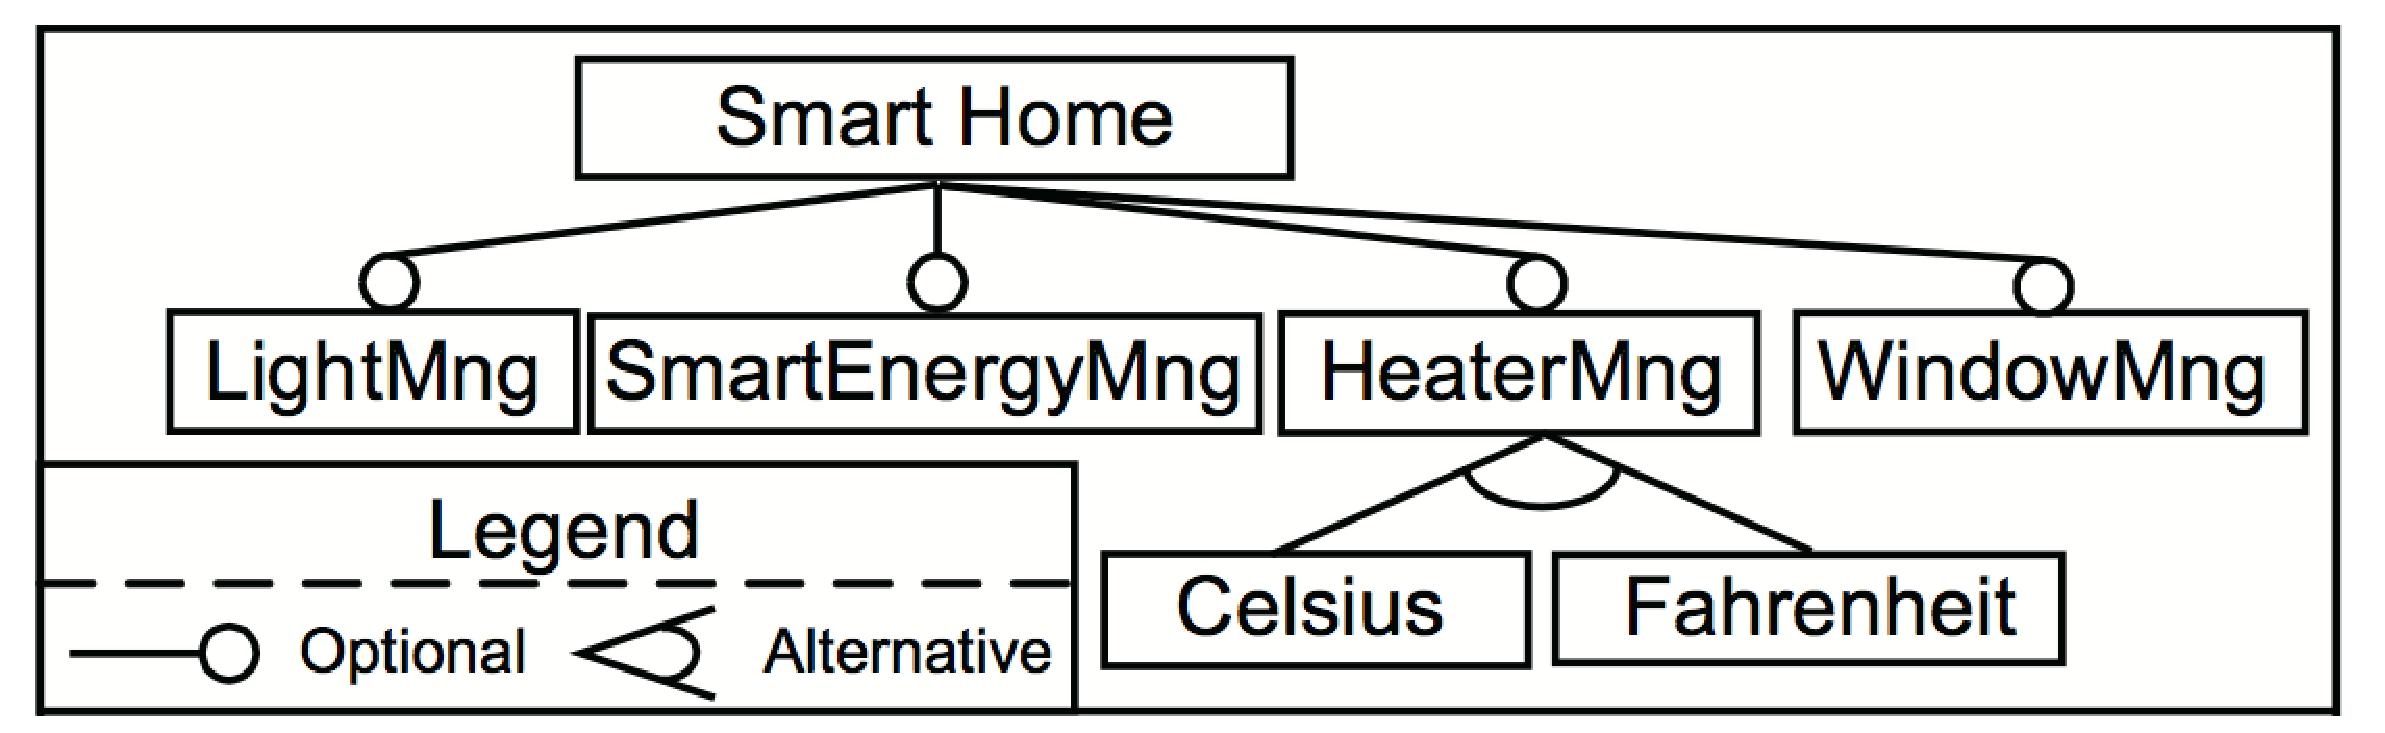
\includegraphics[scale=0.3]{background/simpleSmarthome.eps}
    \caption{�rbol de caracter�sticas simple para nuestro caso de estudio}
    \label{fig:smartHomeFMsimple}
\end{figure}

La Figura~\ref{fig:smartHomeFMsimple} muestra como ejemplo un �rbol de caracter�sticas que especifica la variabilidad inherente a nuestro caso de estudio, sin considerar que las plantas y habitaciones puedan configurarse de manera individual. El �rbol representa un hogar inteligente definido por las siguientes caracter�sticas: controlador de luz, controlador de temperatura, controlador de ventanas y controlador de la energ�a. Tal como se puede ver en la leyenda de la figura, todas estas caracter�sticas son opcionales, es decir, podemos decidir si queremos que est�n o no presentes en el hogar inteligente que generemos. Adem�s, para la caracter�stica ''controlador de temperatura" se ha de especificar una de las dos opciones alternativas que se plantean: grados celsius o grados fahrenheit.

El modo de representaci�n de los �rboles de caracter�sticas permite especificar cierto tipo de restricciones que pueden resultar necesarias para representar con exactitud el comportamiento del producto que queramos construir. En el caso de la Figura~\ref{fig:smartHomeFMsimple} se puede observar que mediante las relaciones ya se est� modelando la restricci�n que especifica que el controlador de temperatura ha de ser necesariamente de uno de los tipos que se indican en el modelo. Otros tipos de relaciones que pueden incluirse sirven para especificar otras restricciones, por ejemplo la obligatoriedad de seleccionar una caracter�stica o un grupo de ellas.

Sin embargo, si quisi�ramos incluir algunas restricciones m�s complejas, la representaci�n gr�fica de los �rboles de caracter�sticas se queda corta. Por ejemplo, en la Figura~\ref{fig:smartHomeFMsimple} podr�amos querer especificar la restricci�n de que si nuestro hogar inteligente tiene un controlador de energ�a, ha de tener tambi�n un controlador de calefacci�n en grados celsius. Es imposible modelar esta restricci�n con las herramientas de las que los �rboles de caracter�sticas disponen. Es por ese motivo que debe permitirse la posibilidad de especificar restricciones externas al �rbol mediante alg�n tipo de lenguaje textual o gr�fico.

%%=========================================================================================%%
%% NOTA(Pablo): Explicar el modelo creado, indicando las cosas que son variables, las que  %%
%%              son alternativas, etc.                                                     %%
%%              Explicar el problema de las restricciones externas                         %%
%%=========================================================================================%%

\begin{figure}[!tb]
    \centerline{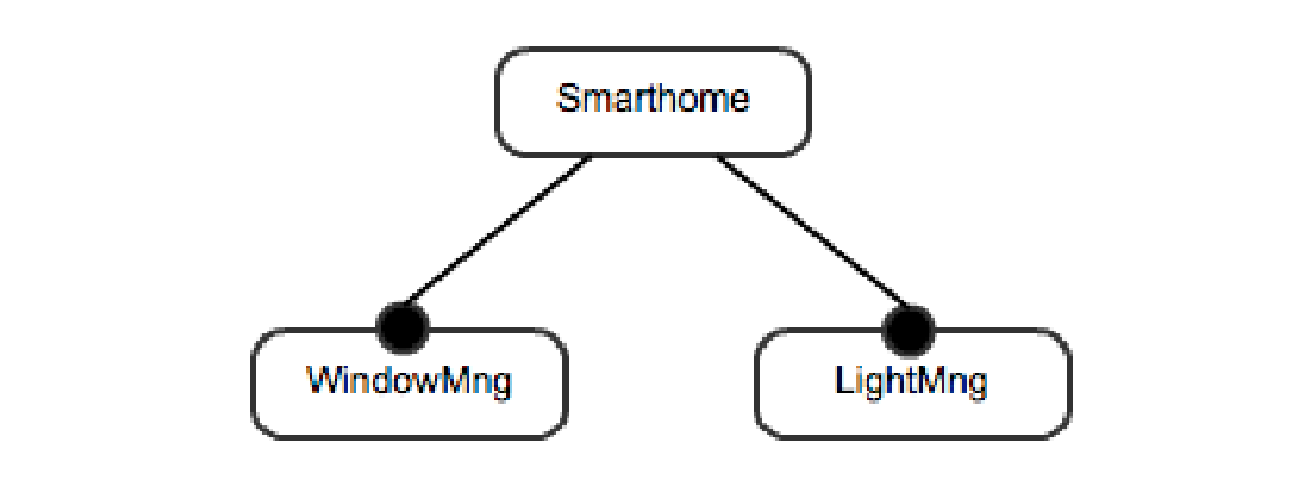
\includegraphics[scale=0.3]{background/simpleSmarthomeConf.eps}}
    \caption{Configuraci�n para la versi�n sencilla del caso de estudio}
    \label{fig:smartHomeConfSimple}
\end{figure}

Una vez creado un �rbol de caracter�sticas para una l�nea de productos software, podemos indicar las caracter�sticas que podemos incluir en un producto software concreto mediante la creaci�n de configuraciones. Una \emph{configuraci�n} no es m�s que una selecci�n v�lida de caracter�sticas. La Figura~\ref{fig:smartHomeConfSimple} muestra en un ejemplo de configuraci�n para el modelo de la Figura~\ref{fig:smartHomeFMsimple} donde se indica que el producto que deseamos construir debe incluir �nica y obligatoriamente un dispositivo de control de luz y un dispositivo de control de ventanas. Obviamente, dicho modelo debe satisfacer las restricciones externas declaradas. 

Los �rboles de caracter�sticas como los anteriormente expuestos no permiten modelar que pueda existir un n�mero variable de ciertas caracter�sticas, como, en nuestro caso, de plantas y habitaciones, y que, adem�s, cada instancia particular de una caracter�sticas pueda  configurarse de forma distinta. Por ejemplo, podr�amos decidir que el sal�n de la casa tenga control inteligente de temperatura, mientras que la cocina, que est� sometida a mayores variaciones de temperatura, no contenga dicha caracter�sticas. Para solventar esta carencia, se introdujeron en los �rboles de caracter�sticas el concepto de caracter�stica clonable. 

\begin{figure}[!tb]
    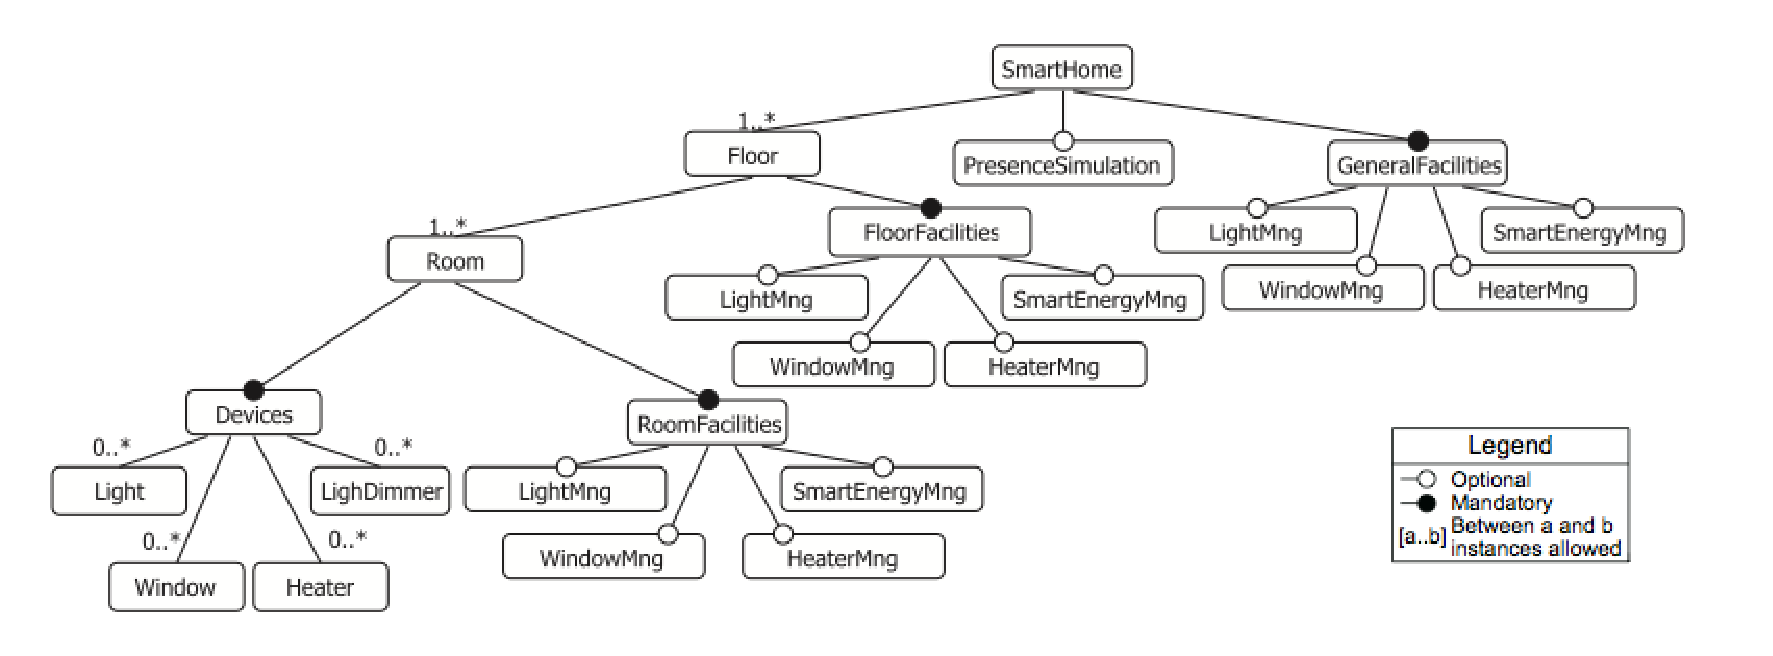
\includegraphics[scale=0.4]{background/featuremodel.eps}
    \caption{�rbol de caracter�sticas completo para nuestro caso de estudio}
    \label{fig:smarHomeFeatureModel}
\end{figure}

La Figura~\ref{fig:smarHomeFeatureModel} muestra el �rbol de caracter�sticas para nuestro caso de estudio incluyendo \emph{caracter�sticas clonables}. Las caracter�sticas \emph{Floor} (Piso) y \emph{Room} (Habitaci�n) son clonables porque pueden aparecer m�s de una vez en las configuraciones creadas. La cardinalidad de ambas caracter�sticas es 1..*, lo que significa que pueden ser seleccionadas de una a infinitas veces. As� mismo, cualquier caracter�stica que sea hija de ellas directa o indirectamente es considerada inmediatamente como caracter�stica. Este es el caso, por ejemplo, de \emph{Devices} y de sus caracter�sticas hijas (\emph{Heater}, \emph{Window}, etc.), que son consideradas clonables tanto por su cardinalidad como por ser hijas de una caracter�stica clonable. 

La repetici�n de las caracter�sticas correspondientes a los diversos controladores (es decir, \emph{WindowMng}, \emph{HeaterMng}, etc.) se debe a que gracias a las caracter�sticas clonables ahora podemos diferenciar los controladores seg�n su colocaci�n y alcance. Es decir, el controlador de temperatura hijo de \emph{RoomFacilities} afectar� s�lo a la habitaci�n a la que pertenezca, el hijo de \emph{FloorFacilities} afectar� al piso al que pertenezca, y el hijo de \emph{GeneralFacilities} afectar� a todo el hogar creado. 
%%=========================================================================================%%
%% NOTA(Pablo): A�adir la figura, si no te entrase bien a lo ancho, mira como meterla 
%%              apaisada en Latex.
%%=========================================================================================%%

A la hora de crear configuraciones para este nuevo �rbol hay que tener en cuenta que podemos seleccionar en m�s de una ocasi�n ciertas caracter�sticas, por lo que necesitamos valernos de alg�n mecanismo que nos permita diferenciarlas entre ellas. El modo de lograrlo es poniendo un nombre a las diferentes selecciones o clones que hagamos de una misma caracter�stica. 

La Figura~\ref{fig:smarthomeCompleteConf} muestra un ejemplo de configuraci�n para el �rbol de caracter�sticas con caracter�sticas clonables de la Figura~\ref{fig:smarHomeFeatureModel}. En ella se puede apreciar que se diferencia entre las diferentes selecciones de la caracter�stica \emph{Floor} poni�ndoles un nombre, en este caso \emph{Ground} (Planta Baja) y \emph{First} (Primer Piso). Del mismo modo con las habitaciones \emph{Kitchen} (Cocina) y \emph{Living} (Sal�n), pertenecientes a la planta baja, y \emph{Bed} (Dormitorio), perteneciente al primer piso. Observando el �rbol de la figura es sencillo comprender qu� elementos y/o controladores tiene instalados cada estancia. Por ejemplo, la cocina est� dotada de dos luces, un regulador de luz, una ventana, un controlador de luz y un controlador de ventanas.

%%=========================================================================================%%
%% NOTA(Pablo): Explicar como se configuran las caracter�sticas clonables usando un 
%%              ejemplo
%%=========================================================================================%%

Como en el caso anterior, las diversas configuraciones no s�lo han de cumplir las restricciones impuestas por el propio �rbol de caracter�sticas, sino tambi�n las restricciones externas. Pero debido a la presencia de caracter�sticas clonables ahora existe un abanico mucho mayor de restricciones posibles que definir. Del mismo modo que antes se pod�an definir diversas restricciones l�gicas ($a implies b$), la presencia de caracter�sticas clonables hace que tambi�n sean necesarias las restricciones num�ricas ($a >= b$), lo que tambi�n a�ade la dificultad de diferenciar qu� caracter�sticas pueden realizar operaciones l�gicas y cuales no. 

Tambi�n es necesaria una operaci�n de contexto que permita aplicar estas restricciones s�lamente a sub�rboles de la configuraci�n. Esto es imprescindible para definir una restricci�n que, por ejemplo, valide que si una habitaci�n tiene un controlador de ventanas, forzosamente ha de tener instalada al menos una ventana. Sin la operaci�n de contexto ser�a imposible saber a qu� caracter�stica \emph{WindowMng} en concreto est� haciendo referencia la restricci�n definida.

El objetivo de este proyecto es implementar un lenguaje textual que haga posible la definici�n de restricciones externas para �rboles de caracter�sticas con caracter�sticas clonables con todas las peculiaridades definidas anteriormente, as� como una herramienta que permita validar si las configuraciones creadas satisfacen o no esas restricciones. 
%%=========================================================================================%%
%% NOTA(Pablo): Explicar el problema de las restricciones cuando incluyen caracter�sticas
%%              clonables y decir que implementar un lenguaje para resolver ese problema 
%%              es el objetivo de este proyecto
%%=========================================================================================%%

%%=========================================================================================%%
%% NOTA(Pablo): Esto no se entiende de forma clara, por lo que se suprime                                         %%
%%=========================================================================================%%
%%
%% Por otro lado, un modelo de caracter�sticas debe poder representar la cardinalidad de 
%% las caracter�sticas, por motivos tanto de comprensi�n (es mucho mejor contar con un 
%% �rbol de 8 nodos que con uno de 100, teniendo ambos un significado equivalente), como 
%% de funcionalidad, ya que permite expresar ciertas restricciones que de no contar con 
%% la cardinalidad no podr�an expresarse.
%% 
%% Adem�s se podr�n disponer de restricciones de usuario m�s complejas, que son las que
%% se han implementado en el editor de especificaci�n y validaci�n de restricciones 
%% desarrollado en este proyecto.
%%
%%=========================================================================================%%

%%=========================================================================================%%
%% NOTA(Pablo): Esto queda obsoleto en el nuevo esquema, por lo cual se suprime            %%
%%=========================================================================================%%
%%
%% La figura \ref{fig7} muestra un ejemplo de modelo de caracter�sticas. En este caso se 
%% trata de un modelo de una casa inteligente o SmartHome, a trav�s del cual, 
%% seleccionando ciertas caracter�sticas u otras podremos construir qu� tipo de casa 
%% queremos. Cada una de las m�ltiples casas diferentes que podamos construir es lo que 
%% se denonima una especializaci�n o configuraci�n de nuestro modelo de caracter�sticas.
%% 
%%  El proceso de crear una configuraci�n a partir de un modelo de caracter�sticas se 
%% conoce como proceso de configuraci�n o proceso de especializaci�n. Consiste en 
%% transformar un modelo de caracter�sticas de tal forma que el modelo resultante sea un
%%  subconjunto de las posibles configuraciones denotadas por el primer modelo. La figura 
%% \ref{fig8} muestra una posible configuraci�n para el modelo de caracter�sticas de la figura %% \ref{fig7}.
%%
%% La relaci�n entre un diagrama de caracter�sticas y una configuraci�n es an�loga a la
%% existenteentre una clase y una de sus instancias en programaci�n orientada a objetos.
%%
%%=========================================================================================%%

\begin{figure}[!tb]
    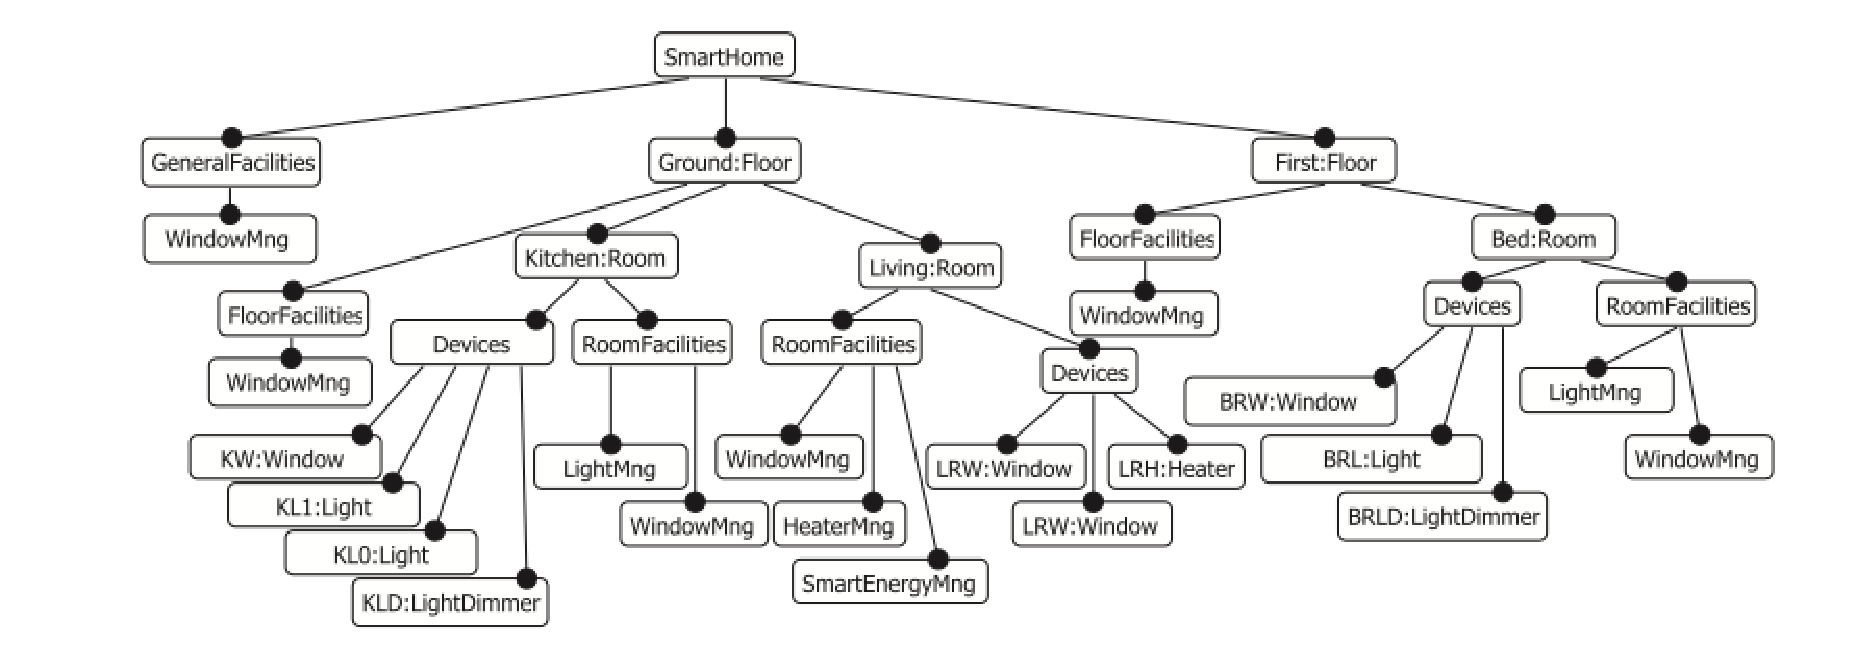
\includegraphics[scale=0.4]{background/configuration.eps}
    \caption{Posible modelo de configuraci�n de una casa inteligente concreta}
    \label{fig:smarthomeCompleteConf}
\end{figure}

\begin{figure}[!tb]
    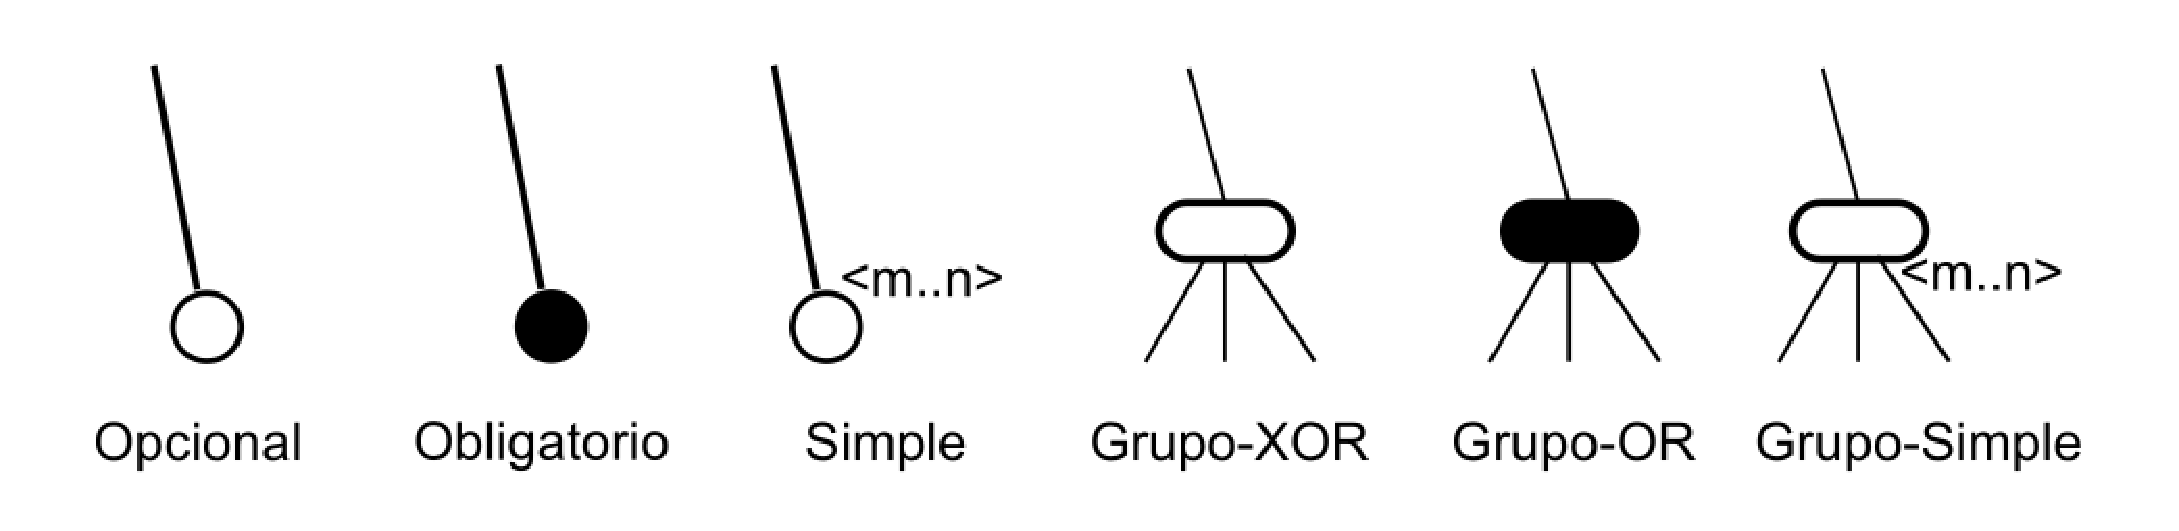
\includegraphics[scale=0.35]{background/relations.eps}
    \caption{Tipos de relaciones entre caracter�sticas }
    \label{fig:relacionesFeatures}
\end{figure}

A modo de resumen, la Figura~\ref{fig:relacionesFeatures} muestra las posibles relaciones que pueden entre caracter�sticas, as� como su representaci�n gr�fica. Dichas relaciones se describen a continuaci�n:

\begin{description}
    \item[Opcional] La caracter�stica hija puede estar o no estar seleccionada
    \item[Obligatoria] La caracter�stica siempre debe estar seleccionada.
    \item[Clonable] La caracter�stica tendr� una cardinalidad $<m,n>$, siendo m y n n�meros enteros que denotan el m�nimo y el m�ximo respectivamente de caracter�sticas que podemos seleccionar.
    \item[Grupo-xor] S�lo una de las caracter�sticas pertenecientes al grupo puede ser seleccionada.
    \item[Grupo-or] Debemos seleccionar como m�nimo una de las subcaracter�sticas, pudiendo seleccionar m�s si lo deseamos.
    \item[Grupo con cardinalidad] El n�mero m�nimo y m�ximo de caracter�sticas a seleccionar dentro del grupo vendr� determinado por su cardinalidad $<m,n>$.
\end{description}

Tras esta secci�n se han proporcionado al lector lo necesario para comprender el contexto del problema que este Proyecto Fin de Carrera pretende resolver. Las siguientes secciones est�n destinadas a explicar las tecnolog�as concretas que se han utilizado para implementar el lenguaje que da soluci�n a los problemas planteados. 


\section{Arquitectura de plugins de Eclipse}
\label{sec:back:eplugins}
%%==================================================================%%
%% Author : Tejedo Gonz�lez, Daniel                                 %%
%%          S�nchez Barreiro, Pablo                                 %%
%% Version: 1.0, 18/11/2012                                         %%                   
%% Version: 1.0, 06/02/2013                                         %%                   
%%                                                                  %%
%% Memoria del Proyecto Fin de Carrera                              %%
%% Antecedentes, arquitectura de plugins de eclipse                 %%
%%==================================================================%%

El entorno de desarrollo Eclipse es un ejemplo de arquitectura modular f�cilmente extensible mediante una compleja, pero sencilla para el programador, arquitectura de \emph{plug-ins}. Un \emph{plug-in} en Eclipse es un componente que provee un cierto tipo de servicio dentro del contexto del espacio de trabajo de Eclipse. Es decir, una herramienta que se puede integrar en el entorno Eclipse junto con sus otras funcionalidades. Dado que la herramienta \emph{Hydra} fue dise�ada como un \emph{plug-in} para Eclipse, y nuestro editor pretende integrarse tanto en \emph{Hydra} como en \emph{Eclipse}, es necesario conocer y manejar el funcionamiento de la arquitectura de plug-ins de Eclipse.

Aunque la arquitectura de plug-ins de Eclipse tiene mucha profundidad y ofrece muchas posibilidades, es imprescindible el dominio de dos de sus conceptos clave para poder trabajar con ella: las dependencias y los puntos de extensi�n. Mediante las dependencias podemos indicar que el plug-in a desarrollar tiene que incorporar toda la funcionalidad y estructura de otro plug-in (en este caso nuestro editor tiene, entre otras, una dependencia con el plug-in de la herramienta Hydra original). Un punto de extensi�n permite a�adir cierta funcionalidad al plug-in desarrollado mediante la inclusi�n autom�tica de ciertos segmentos de c�digo. Un ejemplo cl�sico de punto de extensi�n, y que adem�s ha sido utilizado en el transcurso de este proyecto, es el que permite a�adir un bot�n a la barra de tareas de Eclipse de manera autom�tica, teniendo que implementar �nicamente el c�digo del manejador de ese bot�n.

 \begin{figure}[!tb]
    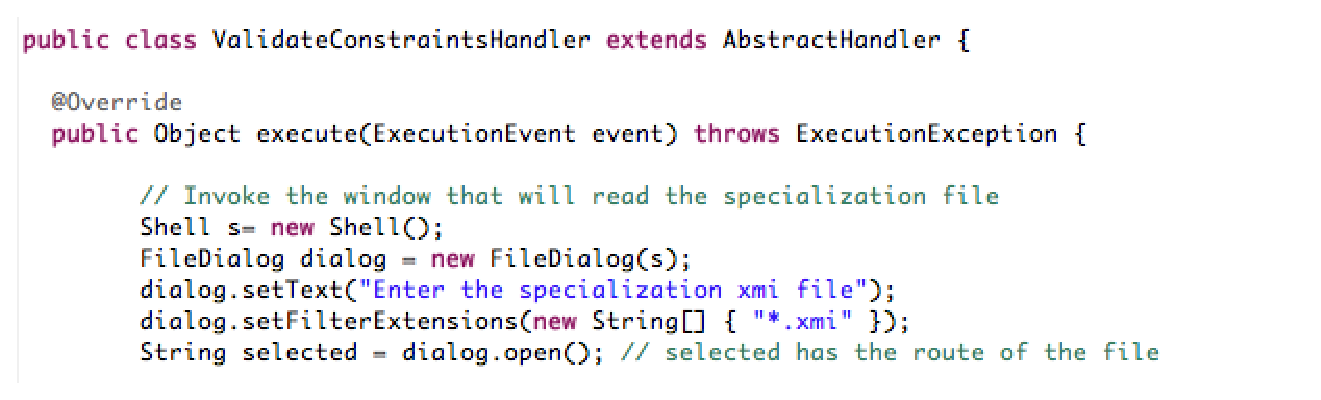
\includegraphics[scale=0.4]{background/codigoManejador.eps}
    \caption{Trozo de c�digo del manejador de un bot�n introducido mediante un punto de extensi�n}
    \label{fig:codigoManejador}
\end{figure}

%%==============================================================================================%%
%% NOTA(Pablo): Esto no se entiende nada
%%==============================================================================================%%
%%
%% En particular, se han utilizado mucho los puntos de extensi�n. Un punto de extensi�n en un
%% plug-in indica la posibilidad de que ese plug-in sea a su vez parte de otro, o que haya 
%% otros plug-ins que sean parte de �l. Esta particularidad permite no s�lo la integraci�n de 
%% nuestro editor con Hydra, sino tambi�n la personalizaci�n de men�s y botones para �l 
%% gracias a la creaci�n de puntos de extensi�n con plug-ins de creaci�n de men�s y barras de
%% herramientas.
%%
%%==============================================================================================%%

%%==============================================================================================%%
%% NOTA(Pablo): Para solucionar
%% - Describir en uno o dos p�rrafos c�mo funciona la arquietctura de plug-ins para Eclipse
%% - Poner un ejemplo de punto de extensi�n, sencillo y concreto, y explicar como funciona 
%%   el punto de extensi�n utilizando algo de c�digo.
%% Si no sabes como escribir esta secci�n, la eliminas directamente, y actualizas la intro 
%% al Cap�tulo de forma conveniente.
%%==============================================================================================%%
